\documentclass{article}
\usepackage{tikz}

\begin{document}

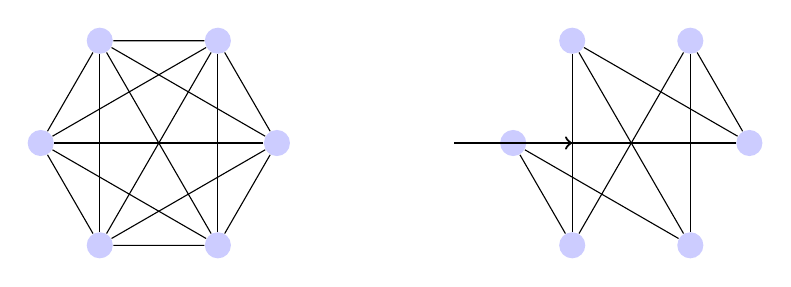
\begin{tikzpicture}[scale=1.5]
    % Define nodes
    \foreach \i in {1,...,6} {
        \node[circle, fill=blue!20] (n\i) at ({(\i-1)*360/6}:1) {};
    }
    
    % Draw edges for the first graph
    \draw (n1) -- (n2);
    \draw (n1) -- (n3);
    \draw (n1) -- (n4);
    \draw (n1) -- (n5);
    \draw (n1) -- (n6);
    
    \draw (n2) -- (n3);
    \draw (n2) -- (n4);
    \draw (n2) -- (n5);
    \draw (n2) -- (n6);
    
    \draw (n3) -- (n4);
    \draw (n3) -- (n5);
    \draw (n3) -- (n6);
    
    \draw (n4) -- (n5);
    \draw (n4) -- (n6);
    
    \draw (n5) -- (n6);
    
    % Draw the second graph
    \begin{scope}[xshift=4cm]
        \foreach \i in {1,...,6} {
            \node[circle, fill=blue!20] (m\i) at ({(\i-1)*360/6}:1) {};
        }
        
        \draw (m1) -- (m2);
        \draw (m1) -- (m3);
        \draw (m1) -- (m4);
        
        \draw (m2) -- (m5);
        \draw (m2) -- (m6);
        
        \draw (m3) -- (m5);
        \draw (m3) -- (m6);
        
        \draw (m4) -- (m5);
        \draw (m4) -- (m6);
    \end{scope}
    
    % Draw the arrow between the two graphs
    \draw[->, thick] (2.5,0) -- (3.5,0);
\end{tikzpicture}

\end{document}